\documentclass[10pt]{article}
\usepackage[margin=0.85in]{geometry}
\usepackage{amsmath,amssymb,bm}
\usepackage{booktabs}
\usepackage{graphicx}
\usepackage{enumitem}
\usepackage[hidelinks]{hyperref}
\usepackage{caption}
\usepackage{titlesec}
\titlespacing*{\section}{0pt}{10pt}{4pt}
\titlespacing*{\subsection}{0pt}{8pt}{3pt}
\captionsetup{font=small,labelfont=bf,skip=4pt}
\setlist{itemsep=2pt,topsep=3pt,leftmargin=1.4em}
\setlength{\parskip}{2pt}
\newcommand{\Tr}{\mathrm{Tr}}
\newcommand{\gl}{\mathfrak{gl}}
\newcommand{\su}{\mathfrak{su}}
\newcommand{\g}{\mathfrak{g}}
\newcommand{\h}{\mathfrak{h}}
\newcommand{\n}{\mathfrak{n}}
\newcommand{\Wg}{\mathcal{W}}
\newcommand{\bPsi}{\bar\Psi}
\newcommand{\bQ}{\bar Q}
\newcommand{\Alt}{\mathrm{Alt}}
\title{\vspace{-1.5cm}\Large\textbf{Fermionic Matrix Models, Fortuity, and the Bootstrap}\vspace{-6pt}}
\author{}
\date{}

\begin{document}
\maketitle
\vspace{-1.0cm}
\begin{center}\begin{minipage}{0.95\textwidth}\small
\textbf{Abstract.} We study a three-parameter family of purely fermionic gauge quantum mechanics, $p$ flavours of
adjoint matter for a rank-$r$ algebra with a nilpotent supercharge of odd degree $q$, using two methods whose
strengths are complementary. Exact cohomology answers questions about which states are BPS: because $Q$ acts on
the Fock space as multiplication by a fixed $q$-form, the maximal irrep factorises over Cartan sites and its BPS
window has width $W=r(w_s-1)+1$ in closed form, where the slot width $w_s$ takes only the values $q-1$, $q$ and
$q+1$ and is controlled by the symmetry type of one bilinear form. A combinatorial criterion based on critical
sets gives a lower bound on $W$ at every weight, and exact integer linear algebra over a weight decomposition,
followed by Kostant inversion, gives BPS multiplicities irrep by irrep for $N$ up to $5$. Since
$\mathcal N=2$ SYK is the $N=1$ member of the same family, R-charge concentration becomes a statement about
rank: it holds for $r\le q-1$ and fails otherwise. The same empty-triangle criterion settles fortuity: an
embedded BPS state is never closed at the next rank, so no class is monotone, and fortuity and concentration
respond to enlarging the gauge group with opposite signs. None of this reaches the density of states, which is
what distinguishes a chaotic model with a super-Schwarzian tail from a solvable one, and for that we turn to a
sector-resolved bootstrap, which supplies rigorous energies where exact diagonalisation cannot, though it does
not yet reach the near-BPS regime either. A semidefinite programme over linear functionals, formulated exactly at finite $N$ in
terms of trace words, gives rigorous lower bounds on the sector ground energies, reproduces them exactly in
every gapped sector at $N=2$ but the almost-BPS one, and points to the closed form $E_0(k;N)=16N^3-(15+38k)N$,
which we prove for all $k\le\lfloor N^2/4\rfloor$: in these sectors the particles fill the lowest adjoint band
with mutually commuting matrix wavefunctions and do not interact. Adding the BPS conditions turns the same programme into a certificate of absence, and
resolving it by gauge Casimir makes the two methods meet: at $N=3$ the exclusion margin in the
maximal-Casimir irrep decays monotonically through $k=8,9,10,11$ and vanishes precisely at $k=12$, which is
where the exact cohomology places the edge of the window. Exact diagonalisation of the zero-weight blocks,
which contain every irrep, gives the sector energies up to the window at $N=3$: the states there lie in irreps
of small Casimir, the maximal irrep being a set of decoupled sites with a gap of one, and the energies rise faster
than the super-Schwarzian $q^2$ law at these sizes. We close with the single-trace forms of $H$, $Q$ and
$\hat C_2$, and with the demonstration that the three-flavour Hamiltonian is not a function of Casimirs, which
is what forces the bootstrap to be sector-resolved in the first place.
\end{minipage}\end{center}
\vspace{8pt}

\section{Introduction}\label{sec:intro}

\subsection{The models}

Let $\g$ be a reductive Lie algebra of rank $r$ and let $\Psi^a$, $a=1,\dots,p$, be complex fermions valued in
$\g$. For $\g=\gl(N)$ we write $\Psi^a_{ij}$ with
$\{\Psi^a_{ij},\bPsi^b_{kl}\}=\delta^{ab}\delta_{il}\delta_{jk}$, the gauge group acting by conjugation. The
Fock space is the exterior algebra
\begin{equation}
\mathcal H=\Lambda^\bullet V,\qquad V=\mathbb C^p\otimes\g,\qquad n\equiv\dim V=p\dim\g,
\end{equation}
graded by the R-charge $k=N_\Psi=\Tr\Psi^a\bPsi^a$. All dynamics comes from one supercharge,
\begin{equation}
Q=\sum_{a_1,\dots,a_q=1}^{p}C_{a_1\cdots a_q}\,\Tr\!\big[\Psi^{a_1}\cdots\Psi^{a_q}\big],\qquad
H=\{Q,\bQ\}\ \ge0,\qquad [N_\Psi,Q]=q\,Q .
\label{eq:Q}
\end{equation}
The flavour sum runs over all tuples. Moving an odd matrix around the trace costs $(-1)^{q-1}=+1$, so the trace
is cyclically but not totally antisymmetric in the flavours and only the cyclic-invariant part of $C$
contributes; terms with repeated flavours such as $\Tr[\Psi^1\Psi^1\Psi^2]$ are non-zero. Only odd $q$ is
admissible, for two reasons: a cyclic shift gives $\Tr[\Psi^q]=(-1)^{q-1}\Tr[\Psi^q]$, so the trace vanishes
identically for even $q$; and $Q^2=0$ requires the exchange of the two $q$-tuples in $C\otimes C$, a permutation
of $2q$ fermions built from $q^2$ transpositions, to produce a relative sign.

Every $\Psi$ is a creation operator, so $Q$ contains no annihilators and acts on $\Lambda^\bullet V$ as plain
left multiplication,
\begin{equation}
Q=\omega\wedge-\,,\qquad \omega=\sum C_{a_1\cdots a_q}\Tr[\Psi^{a_1}\cdots\Psi^{a_q}]\in\Lambda^qV,
\qquad H^\bullet=\ker Q/\operatorname{im}Q .
\label{eq:wedge}
\end{equation}
Nilpotency is then automatic for odd $q$, since $\omega\wedge\omega=-\omega\wedge\omega$, and survives any
change of couplings or of index structure. Concretely, $\ker Q$ is the set of states that $\omega$ annihilates
and $\operatorname{im}Q$ the set it produces, and $\operatorname{im}Q\subseteq\ker Q$ is precisely $Q^2=0$. The
whole BPS problem is therefore the cohomology of multiplication by one specific element of $\Lambda^qV$. It is
worth seeing this once on the object that recurs below: on $\Lambda^\bullet\mathbb C^3$ with
$\omega=e_1\wedge e_2\wedge e_3$ the top form, $\ker Q=\Lambda^{\ge1}$ of dimension $7$ and
$\operatorname{im}Q=\Lambda^3$ of dimension $1$, so the cohomology is $\Lambda^1\oplus\Lambda^2$ with Poincar\'e
polynomial $3t+3t^2$, which is the single-site factor that gives $27,81,81,27$ at $N=3$.

\subsection{SYK is the member at $N=1$}

The family is usually presented as a matrix generalisation of SYK, but SYK is already inside it. At $N=1$ the
matrices are $1\times1$, the trace is the identity map, and \eqref{eq:Q} becomes
$Q=\sum_{a_1<\cdots<a_q}C_{a_1\cdots a_q}\psi^{a_1}\cdots\psi^{a_q}$ with $C$ now totally antisymmetric, which
is $\mathcal N=2$ SYK with $p$ complex fermions. The gauge algebra is $u(1)$, whose adjoint action is trivial,
so nothing constrains $C$; this is why the SYK coupling is free while the matrix coupling is not. Randomness
plays no role in what follows: what a Gaussian ensemble supplies is genericity, and genericity is optimal here
because matrix ranks are lower semicontinuous in $\omega$, so specialising the couplings can only enlarge the
cohomology. We checked the identification rather than assuming it, running the full matrix machinery at $N=1$
against a bare generic $q$-form and finding identical Betti numbers for every $p$ from $4$ to $12$.

What varies along the family is not the coupling tensor but the interaction hypergraph. Calling a
\emph{triangle} the support of a non-zero term of $\omega$, SYK has all $\binom pq$ of them, whereas at general
$N$ only the index-loop triangles survive out of the $\binom{pN^2}{q}$ available, a fraction of order $6/N^3$ at
$q=3$. The parameter $N$ dials the hypergraph from complete to sparse.

\subsection{What each method is for}

The Cartan torus acts on $\Psi_{ij}$ by $u_iu_j^{-1}$, so that mode carries weight $e_i-e_j$ and a state's
weight is the row sums minus the column sums of its occupation matrix. Since $Q$ is a gauge singlet it preserves
the weight, and since $[N_\Psi,Q]=qQ$ it raises $k$ by $q$, so the cohomology splits into complexes labelled by
a $U(N)$ irrep $\lambda$, a flavour charge, and $c=k\bmod q$. R-charge concentration, in the sense of Chang,
Chen, Sia and Yang \cite{CCSY}, says that in each complex of macroscopic index all BPS states sit at one degree.
Writing $W$ for the number of consecutive R-charges carrying BPS states, concentration requires $W\le q$, since
a window wider than the grading period must put two occupied degrees in one residue class.

Section \ref{sec:bps} answers that question with exact methods. Cohomology is the right tool there because the
BPS condition is cohomological, the complexes are finite-dimensional, and the answer is an integer that exact
linear algebra can certify. What cohomology cannot see is energy. It says which states have $E=0$ and says
nothing whatever about the states just above, and it is the density of states near the BPS edge that
distinguishes a chaotic model with a near-BPS super-Schwarzian tail \cite{TW} from a solvable one with a gap
fixed by a Casimir. Section \ref{sec:bootstrap} therefore turns to a sector-resolved bootstrap, which produces
rigorous lower bounds on $E_0$ in each R-charge sector and, when the gauge Casimir is added as a linear
constraint, in each irrep. The two methods then meet: the bootstrap's BPS-exclusion margin, computed with no
knowledge of the cohomology, vanishes exactly where the cohomology places the edge of the window. Exact
diagonalisation in symmetry-resolved blocks then supplies the energies next to the window at $N=3$, which the
bootstrap does not yet reach.

\section{BPS spectra and the R-charge window}\label{sec:bps}

\subsection{Irreps and the maximal weight}

\begin{figure}[t]\centering
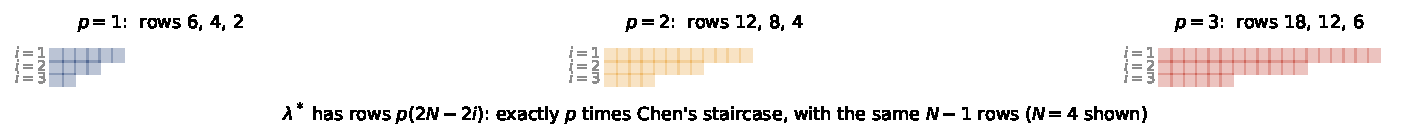
\includegraphics[width=0.94\textwidth]{report_figs/g_staircase.pdf}
\caption{The highest weight occurring in the Fock space, shifted to a partition. Adding flavours stretches the
rows without producing new ones, so $\lambda^*$ has the same $N-1$ rows for every $p$.}
\label{fig:staircase}
\end{figure}

Since each mode has weight $e_i-e_j$ of total zero, only weights with $\sum_i\lambda_i=0$ occur, and the
occurring dominant weights are exactly those dominated by the maximal one. The maximal weight itself is found
greedily, filling row $1$ and emptying column $1$, then row $2$, and so on:
\begin{equation}
\lambda^*_i=p\,(N+1-2i),\qquad
C_2^{\max}=\tfrac12 p(p+1)\textstyle\sum_i(N+1-2i)^2=\frac{p(p+1)N(N^2-1)}{6},
\label{eq:lamstar}
\end{equation}
using $\lambda^*_i+N+1-2i=(p+1)(N+1-2i)$ and $\sum_i(N+1-2i)^2=N(N^2-1)/3$. At $p=1$ this is $N(N^2-1)/3$, which
is Chen's $C_2(r_*)$, so \eqref{eq:lamstar} is its multi-flavour generalisation; at $p=3$ it gives
$2N(N^2-1)=48,120,240$ for $N=3,4,5$. Shifting $\lambda^*$ to a partition gives row lengths $p(2N-2i)$, exactly
$p$ times Chen's staircase with the same $N-1$ non-empty rows (Fig.~\ref{fig:staircase}). Counting the occurring
irreps gives $25$ at $N=3$, $213$ at $N=4$ and $2131$ at $N=5$; the box bound $|\lambda_i|\le p(N-1)$ is
necessary but not sufficient, and dominance is the exact criterion.

\subsection{Index loops and the width at the maximal weight}

\begin{figure}[t]\centering
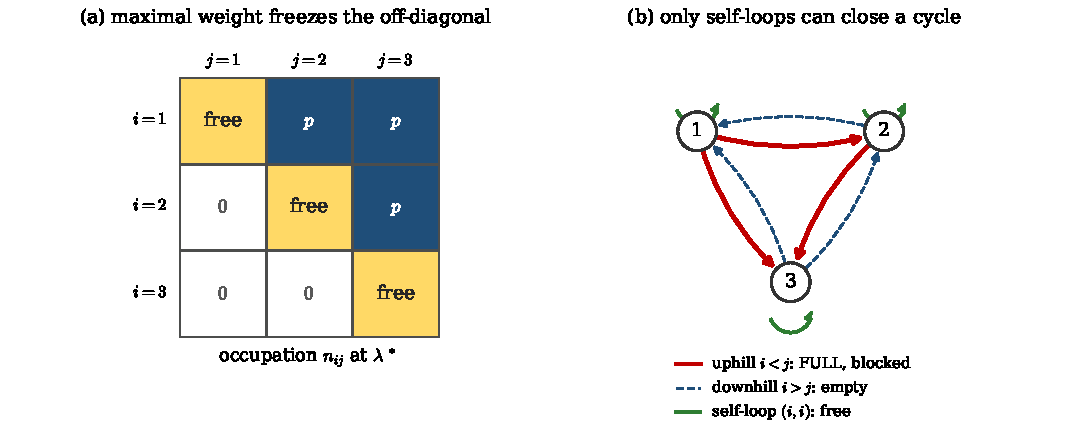
\includegraphics[width=0.93\textwidth]{report_figs/g_loops.pdf}
\caption{(a) At the maximal weight the occupation is forced: every mode with $i<j$ is full, every mode with
$i>j$ is empty, and only the diagonal is free. (b) Reading modes as coloured directed edges, $Q$ creates a
closed walk $i\to j\to k\to i$ and needs all its edges empty. Uphill edges are occupied, so every creatable step
is non-increasing; a cycle of non-increasing steps must be constant, leaving only self-loops.}
\label{fig:loops}
\end{figure}

At $\lambda^*$ the off-diagonal sector is rigid, so the weight space is an exterior algebra on the zero-weight
modes, $(\Lambda V)_{\lambda^*}\cong\Lambda^\bullet(\mathcal Z)$ with $\mathcal Z=\h\otimes\mathbb C^p$ of
dimension $pr$. Which terms of $Q$ survive is best seen graphically. Read a mode $\Psi^a_{ij}$ as a directed
edge $i\to j$ of colour $a$. A term is a trace, so the $q$ modes it creates form a closed walk, and Pauli
exclusion lets it act only if every edge of that walk is empty. At the maximal weight the empty modes are
exactly those with $i>j$, together with free diagonal flavours, so every step of a creatable walk satisfies
$i_t\ge i_{t+1}$: the walk may descend or stay level but never climb, because all uphill edges are occupied.
Closing it forces $i_1=\cdots=i_q$. Only self-loops survive, meaning $q$ diagonal modes of distinct flavours at
a single site, which we verified exhaustively at $N=3$, $p=3$, where all $192$ non-zero actions of $Q$ on the
maximal-weight space are of that form.

Because every surviving term sits at one site, $Q=\sum_{i=1}^rQ_i$ with $Q_i=\omega_{\rm sl}\wedge$ on
$\Lambda^\bullet\mathbb C^p$ and $\omega_{\rm sl}=\Alt(C)$, the $q$ creation operators of a self-loop being at
the same site and anticommuting. The $Q_i$ act on disjoint tensor factors of
$\Lambda(\mathcal Z)=(\Lambda^\bullet\mathbb C^p)^{\otimes r}$, so K\"unneth applies and Poincar\'e polynomials
multiply,
\begin{equation}
Z_{\max}(t)=t^{k_0}\big(z_{\rm slot}(t)\big)^{r},\qquad
z_{\rm slot}(t)=\sum_j\dim H^j\big(\Lambda^\bullet\mathbb C^p,\ \omega_{\rm sl}\wedge\big)t^j,
\label{eq:kunneth}
\end{equation}
with $k_0=p|\Delta^+|$ the number of frozen off-diagonal modes. Multiplying $r$ copies adds degree spans, so if
$z_{\rm slot}$ is supported on $w_s$ degrees then
\begin{equation}
W=r\,(w_s-1)+1 .
\label{eq:ranklaw}
\end{equation}
It is worth running this once. At $p=q=3$ and $N=3$ the slot algebra has dimensions $1,3,3,1$ and $\Alt(C)$
spans the one-dimensional $\Lambda^3\mathbb C^3$, so $\omega_{\rm sl}\wedge$ is non-zero only as
$\Lambda^0\to\Lambda^3$; hence $H^0=0$, $H^1=H^2=3$, $H^3=0$, and $z_{\rm slot}=3t(1+t)$. Cubing and restoring
the prefactor gives $Z_{\max}=27t^{12}+81t^{13}+81t^{14}+27t^{15}$, in exact agreement with computation.

\begin{table}[t]\centering\small
\begin{tabular}{llrl}
\toprule
$N$ & window ($N_\Psi$) & $W$ & BPS multiplets $h^k$\\
\midrule
2 & $5,6,7$ & 3 & $9,\ 18,\ 9$\\
3 & $12,\dots,15$ & 4 & $27,\ 81,\ 81,\ 27$\\
4 & $22,\dots,26$ & 5 & $81,\ 324,\ 486,\ 324,\ 81$\\
5 & $35,\dots,40$ & 6 & $243,\ 1215,\ 2430,\ 2430,\ 1215,\ 243$\\
\bottomrule
\end{tabular}
\caption{Exact BPS multiplets of the maximal irrep at $p=q=3$, as predicted by \eqref{eq:kunneth}: $3^N\binom Nj$
over $N+1$ consecutive charges centred on $pN^2/2$, totalling $6^N$. The factor $(1+t)^N$ is the same one that
appears in Chen's single-matrix $Z_{\rm BPS}$.}
\label{tab:profiles}
\end{table}

\subsection{What this says about SYK}

\begin{figure}[t]\centering
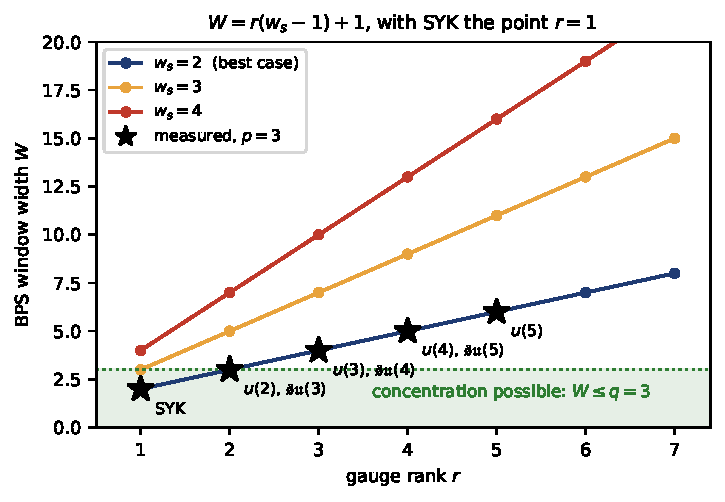
\includegraphics[width=0.52\textwidth]{report_figs/g_ranklaw.pdf}
\caption{The rank law with the measured models on it. SYK is not a separate case but the point $r=1$;
concentration survives exactly as far as rank two.}
\label{fig:ranklaw}
\end{figure}

Setting $r=1$ in \eqref{eq:ranklaw} gives $W=w_s$, and $r=1$ is the $N=1$ member, so the rank law already
contains SYK. This is not a coincidence of notation: $z_{\rm slot}$ is by definition the cohomology of a generic
$q$-form on $\mathbb C^p$, which is the SYK computation. One formula therefore covers both ends of the family,
and concentration becomes the condition
\begin{equation}
r\,(w_s-1)\ \le\ q-1 .
\label{eq:conc-rank}
\end{equation}
Every model we have measured has $W=r+1$, including SYK (Fig.~\ref{fig:ranklaw}). That $u(2)$ and $\su(3)$,
different algebras of different $N$ and different dimension, give the same $W$ is a non-trivial check that rank
rather than $N$ or $\dim\g$ is the governing variable.

\subsection{The slot width takes three values}

Everything reduces to $w_s$. Grade $\Lambda^\bullet\mathbb C^p$ by $j$ mod $q$ and let
\begin{equation}
E_c=\sum_{j\equiv c\ (q)}(-1)^j\binom pj=\frac1q\sum_{m=0}^{q-1}\zeta^{-mc}(1-\zeta^m)^p,\qquad
\zeta=e^{2\pi i/q},
\label{eq:index}
\end{equation}
be the Witten index of class $c$, a topological invariant independent of the coupling. Since
$\sum_cE_c=(1-1)^p=0$, exactly one non-zero $E_c$ is impossible, and since no factor $1-\zeta^m$ vanishes they
cannot all be zero, so at least two classes carry cohomology. This gives $w_s\ge2$ and hence $W\ge r+1$:
concentration already requires $r\le q-1$ whatever the flavour content.

Computation says more. For generic couplings every class with $E_c\ne0$ carries cohomology in a single degree,
of dimension exactly $|E_c|$, with no exception in twenty-seven cases checked class by class at $q=3,5,7$. At
most one class ever has $E_c=0$, and it is either empty or carries two degrees, so
\begin{equation}
w_s=\begin{cases} q-1,&\text{the zero-index class is empty},\\
q,&\text{no class has vanishing index},\\
q+1,&\text{the zero-index class is occupied}.\end{cases}
\label{eq:trichotomy}
\end{equation}
Which case occurs is settled by a connecting homomorphism. Adjoining one flavour writes
$\omega_{p+1}=\alpha+e\wedge\beta$ and, using that $\beta$ has even degree while $\alpha$ has odd degree,
\begin{equation}
\omega_{p+1}\wedge(x+e\,y)=\alpha x+e\,(\beta x-\alpha y),
\end{equation}
so the new complex is two copies of the old one glued by $\beta$. Since $q(q-1)$ is even, $\alpha$ and $\beta$
commute and $\beta$ descends to $\delta:H^j_p\to H^{j+q-1}_p$, the connecting map of the resulting long exact
sequence. It raises degree by $q-1$, hence sends class $c$ to class $c-1$, and can be non-zero only between two
occupied degrees exactly $q-1$ apart. When $w_s=q$ there is precisely one such map, and particle-hole
conjugation puts its source and target at $j$ and $p-j$ with $j=\frac12(p-q+1)$, so they are Poincar\'e dual and
$\delta$ is a bilinear form,
$\langle a,b\rangle_\delta=[\beta\wedge a\wedge b]$, with
$\langle b,a\rangle_\delta=(-1)^j\langle a,b\rangle_\delta$. A generic symmetric form is non-degenerate, so
$w_s$ drops to $q-1$; an antisymmetric form on an odd-dimensional space cannot be, so $w_s$ rises to $q+1$.
Hence $w_s$ cycles through $q-1,q,q+1,q$ with period four in $p$, turning at $p\equiv q+1$ mod $4$. Building
$\delta$ explicitly over $\mathbb F_P$ confirms this in all nine available cases.

Two consequences follow. Since $w_s\ge q-1$, the best available rank law is $W=r(q-2)+1$, so
\eqref{eq:conc-rank} permits rank $2$ at $q=3$ and only rank $1$, that is SYK itself, for every $q\ge5$: the
cubic supercharge is the only degree that tolerates a gauge group. And since $w_s\ge2$ always, a bounded window
with $r\to\infty$ is impossible, so concentration is a property of a family whose parameter, for a matrix model,
must be the rank.

\subsection{A lower bound at every weight}\label{sec:critical}

\begin{figure}[t]\centering
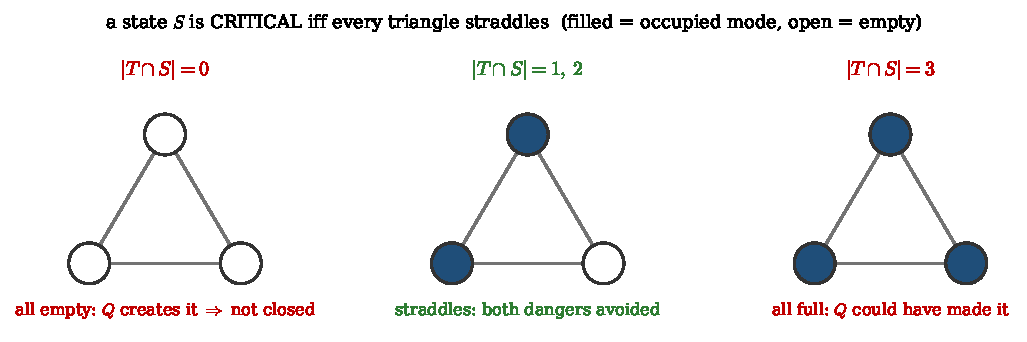
\includegraphics[width=0.93\textwidth]{report_figs/g_critical.pdf}
\caption{The three cases. If a triangle is entirely empty, $Q$ can create it and $S$ is not closed. If it is
entirely occupied, $S$ could have been produced by $Q$ and the non-exactness argument fails. Only straddling
triangles avoid both.}
\label{fig:critical}
\end{figure}

Equation \eqref{eq:ranklaw} is derived at the maximal weight. A weaker statement holds everywhere, by an
elementary argument that also exposes the mechanism. Say that a set of modes $S$ is \emph{critical} if every
triangle meets it partially, $0<|T\cap S|<q$; equivalently, neither $S$ nor its complement contains a triangle.
The two inequalities do different jobs (Fig.~\ref{fig:critical}). The upper one makes $m_S$ closed: for
$\omega_T\wedge m_S$ to be non-zero all $q$ modes of $T$ must be absent from $S$, which criticality excludes, so
every term is Pauli-blocked. The lower one makes $m_S$ non-exact: since $Q$ only ever adds a triangle, the
coefficient of $m_S$ in $\omega\wedge y$ is $\sum_{T\subseteq S}\pm c_T\,y_{S\setminus T}$, and criticality
gives $T\not\subseteq S$ for every triangle, so that sum is empty for every $y$. Each critical set therefore
gives a non-zero class in $H^{|S|}$, and distinct ones give independent classes.

Letting $\alpha$ be the largest triangle-free set and $\tau=n-\alpha$ the transversal number, $S$ is critical
exactly when both $S$ and $S^c$ are hitting sets, so critical sets live in $\tau\le|S|\le n-\tau$ and
\begin{equation}
W\ \ge\ n-2\tau+1\ =\ 2\alpha-n+1 .
\label{eq:taubound}
\end{equation}
Gauge invariance supplies a large triangle-free set for free. Each term of $Q$ is a singlet, so the weights of
its $q$ modes sum to zero, while inside $\n^+\otimes\mathbb C^p$ every mode carries a positive root and a
non-empty sum of positive roots is never zero. No triangle fits in the positive-root subspace, for any reductive
$\g$ and any invariant coupling, so $\alpha\ge\frac12(n-pr)$ and the root contribution cancels in
\eqref{eq:taubound}, leaving $W\ge2\alpha_{\rm cart}-pr+1$ in terms of the Cartan sector alone. For single-trace
$u(N)$ a trace of $q$ diagonal matrices localises to one site, so $\alpha_{\rm cart}=\min(p,q-1)N$ and
\begin{equation}
W\ \ge\ N\big(2\min(p,q-1)-p\big)+1 ,
\label{eq:main}
\end{equation}
which at $p=1$ reads $W\ge N+1$, recovering Chen's single-matrix window combinatorially with no Casimir argument.
The explicit critical sets are $A_{\mathbf s}=\{\text{all }p\text{ flavours of }E_{ij},\ i<j\}\cup\{s_i\text{
flavours of }E_{ii}\}$ with $\max(0,p-q+1)\le s_i\le\min(p,q-1)$: the strictly upper part admits no closed loop
and each site is one flavour short of a self-loop, and the complement is triangle-free for the same reason.

\begin{table}[t]\centering\small
\begin{tabular}{lrrrl}
\toprule
$p$ & $\tau$ (closed form) & $\tau$ (exact integer program) & bound \eqref{eq:main} & measured $W$\\
\midrule
1 & $N(N-1)/2$ & $3,6,10,15$ & $N+1$ & $N+1$ \quad(tight)\\
2 & $pN(N+1)/2-2N$ & $6,12,20$ & $2N+1$ & $2N+1$ \quad(tight)\\
3 & $pN(N+1)/2-2N$ & $5,12,22,35$ & $N+1$ & $N+1$ \quad(tight)\\
4 & $pN(N+1)/2-2N$ & $18$ & $1$ & $2N+1$ \quad(valid, loose)\\
\bottomrule
\end{tabular}
\caption{The transversal number and the resulting bound for single-trace $u(N)$. The closed form agrees with an
exact integer program in all twelve cases tested ($p$ from $1$ to $4$, $N$ from $2$ to $6$). The bound is
attained for $p\le3$; at $p=4$ the family $A_{\mathbf s}$ is no longer optimal.}
\label{tab:tau}
\end{table}

The immediate consequence is a no-go: for $p\le q-1$ we get $W\ge pN+1$, so concentration fails for every
$N>(q-1)/p$, and at $p=q=3$ this reads $W\ge N+1>q$ for all $N\ge3$. Table~\ref{tab:tau} shows the bound against
what is measured.

\subsection{Cohomology irrep by irrep}\label{sec:numerics}

The bound is one thing and the spectrum is another. To get the latter we compute exactly. The complex splits
over weights because $Q$ is a gauge singlet, which replaces the $2^{pN^2}$-dimensional Fock space by weight
spaces of dimension at most a few times $10^4$; within each weight space the ranks of the integer matrices
$Q_k$ are computed by Gaussian elimination over $\mathbb F_P$, with every rank confirmed against a second prime,
and per-irrep multiplicities follow by Kostant inversion of
$\dim H^k(W_\lambda)=\sum_{\mu\ge\lambda}K(\mu,\lambda)h^k_\mu$ from the top down. Two devices extend the reach:
a right-looking blocked LU whose trailing update is a single BLAS matrix multiply, kept exact by choosing the
prime small enough that float64 products are exact integers; and $\mathbb Z_p$ flavour blocking over a field
containing a $p$-th root of unity, which splits each weight space into $p$ blocks and buys a factor of $p^2$ in
both time and memory while resolving the flavour charge for free.

\begin{table}[t]\centering\small
\begin{tabular}{llllrl}
\toprule
$N$ & irreps computed & Casimir range & window & total BPS states & index-invisible\\
\midrule
2 & all 4 & $12$ down to $0$ & $5\ldots7$ & $972$ & $0\%$\\
3 & 13 of 25 & $48$ down to $24$ & $12\ldots15$ & $1\,914\,064$ & $10.1\%$\\
4 & 13 of 213 & $120$ down to $107$ & $22\ldots26$ & $3\,008\,825\,568$ & $19.0\%$\\
5 & maximal only & $240$ & $35\ldots40$ & $6^5=7776$ & n/a\\
\bottomrule
\end{tabular}
\caption{Exact BPS spectra at $p=q=3$, resolved into $U(N)$ irreps. The window is the same set of degrees in
every irrep computed, of width $N+1$ and centred on $pN^2/2$. ``Index-invisible'' is the fraction of BPS states
not accounted for by the refined Witten index, which is a lower bound on the count and equals it only when the
strand is concentrated.}
\label{tab:cohom}
\end{table}

Table~\ref{tab:cohom} collects the results. Three features matter. First, the window is the same in every irrep
computed, not merely at the top: at $N=3$ all thirteen irreps down to $C_2=24$ have support exactly
$\{12,13,14,15\}$, including $(4,0,-4)$ whose Fock multiplicity is $110\,080$, some $215$ times that of the
maximal irrep. Descending the Casimir ladder is what makes this a statement about the spectrum rather than about
its thin top. Second, the index is a lower bound and not a proxy: the excess over the index is $10\%$ at $N=3$
and $19\%$ at $N=4$, so saturation, which is the sharp form of concentration, fails wherever the index is
non-zero. Third, the profile $3^N\binom Nj$ of Table~\ref{tab:profiles} is not a law. It holds for eleven of the
thirteen irreps at $N=4$ and breaks at $C_2=107$, where the profile is $114,1572,2916,1572,114$, with the centre
unchanged and the window edges suppressed. The width is what is robust.

\section{Fortuity}\label{sec:fortuity}

The window is one half of what makes a matrix model a candidate for black-hole microstates; the other is that
its BPS states should be fortuitous rather than monotone, existing at one rank and not lifting from smaller
ones. This section settles that question, and the answer turns out to be governed by the same object as the
window.

For the single-matrix model the BPS states fill $r_*$, whose Young diagram is the staircase with $2N-2i$ boxes
in row $i$ and exactly $N-1$ rows. Going down in rank that diagram has too many rows to exist as a $U(M)$
irrep; going up it is no longer the maximal-Casimir representation. The states therefore exist at one rank
only. By \eqref{eq:lamstar} the diagram of $\lambda^*$ has rows $p(2N-2i)$, with the same $N-1$ rows for every
$p$ (Fig.~\ref{fig:staircase}), so Chen's argument generalises verbatim to all flavour numbers. The difficulty
is that our BPS states are not confined to one irrep: at $N=3$, $p=3$ all thirteen irreps of
Table~\ref{tab:cohom} carry them, each with the same window. A statement about $\lambda^*$ alone therefore
cannot settle fortuity here, and we give a local argument instead, one that works state by state and does not
care which irrep the state sits in.

\begin{figure}[t]\centering
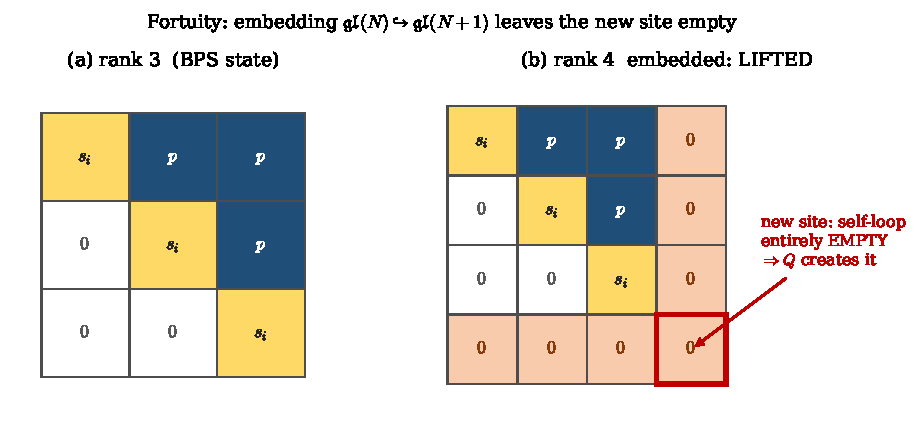
\includegraphics[width=0.85\textwidth]{report_figs/g_fortuity.pdf}
\caption{Embedding $\gl(N)\hookrightarrow\gl(N+1)$ as the upper-left block leaves every mode carrying the new
index unoccupied. The self-loop at the new site is then an entirely empty triangle, so $Q_{N+1}$ creates it and
the state is not closed at the larger rank.}
\label{fig:fortuity}
\end{figure}

Let $\iota$ embed $\gl(N)\hookrightarrow\gl(N+1)$ as the upper-left block. It is worth being careful about what
$\iota$ does and does not give, since it is \emph{not} a chain map: $\omega_{N+1}$ contains terms carrying the
new index that $\iota(\omega_N)$ does not, so $\omega_{N+1}\wedge\iota(m_S)\ne\iota(\omega_N\wedge m_S)$ and no
map on cohomology is induced. This is the observation of Tierz \cite{Tierz}, whose remedy is to compare ranks by
the projection $\pi_{M\to N}$ deleting every monomial that uses an index above $N$, which \emph{is} a chain map,
and to call a class fortuitous when it lies outside the image of the projections from all larger ranks.

What the triangle language of \S\ref{sec:critical} supplies is the sharp local reason the inclusion fails, and
it fails maximally. Under the embedding every mode carrying the index $N+1$ is unoccupied, so the self-loop at
the new site, $T=\{\Psi^{a_1}_{N+1,N+1},\dots,\Psi^{a_q}_{N+1,N+1}\}$ with $q$ distinct flavours, satisfies
$T\cap S=\varnothing$ for any embedded state $S$. A triangle disjoint from $S$ is precisely one that $Q$ can
create, the Pauli blocking that made critical states closed being absent here, so $Q_{N+1}\,\iota(m_S)\ne0$:
the embedded representative is not merely unlifted, it is never closed. For $p<q$ the same holds for the sets
$A_{\mathbf s}$ via the mixed loop $i\to N+1\to j\to i$ with $i<j$, since the two edges through $N+1$ are new
and hence empty while the return edge $(j,i)$ is lower-triangular and hence empty. We verified this at
$p=q=3$, where all $9$ BPS states of rank $2$ and all $27$ of rank $3$ fail to be closed at the next rank, with
the disjoint triangle exhibited in each case. The obstruction is therefore uniform: it removes every BPS state
at once, which is why no stabilisation map exists rather than one that happens to vanish.

There is a tension here worth stating plainly, because it constrains the whole search. Fortuity and
concentration rest on the same object, an empty triangle, and respond to the same structural knob with opposite
signs. Enlarging the gauge group manufactures a fresh site whose self-loop is necessarily empty, which is what
blocks monotony and so produces fortuity; the very same enlargement raises the rank, which by
\eqref{eq:ranklaw} widens the window and destroys concentration. The two properties one wants a fortuitous
matrix model to have therefore pull against each other, which may be why the combination has proved hard to
realise in this family.

\section{Density of states and the bootstrap}\label{sec:bootstrap}

Nothing in Section \ref{sec:bps} says anything about energies above zero. That is the gap the bootstrap fills.

\subsection{The sector-resolved semidefinite programme}

The object of interest is the ground energy $E_0(k)$ of the sector with $N_\Psi=k$. Rather than optimising over
states we optimise over linear functionals $\phi(O)=\Tr[\rho_kP_kOP_k]$, where $\rho_k$ is Hermitian on the
$k$-block and is \emph{not} assumed positive:
\begin{equation}
\begin{gathered}
\min_{\rho_k=\rho_k^\dagger}\ \phi(H)\qquad\text{subject to}\\[3pt]
\phi(\mathbf 1)=1,\qquad
\big[\phi(\Tr w_a^\dagger w_b)\big]_{ab}\succeq0,\qquad
\big[\phi((\Tr w_a)^\dagger\Tr w_b)\big]_{ab}\succeq0,\qquad
\phi([H,X])=0,\qquad \phi((N_\Psi-k)X)=0 .
\end{gathered}
\label{eq:sdp}
\end{equation}
Here $w$ runs over open, adjoint-valued words in the letters $\Psi^a,\bPsi^a$ up to a length $L$ called the
level. The two matrix inequalities are positivity of the Gram matrix of the states $w_{ij}|\psi\rangle$ in its
adjoint and singlet channels; the equalities are the equations of motion and the statement that the functional
lives in sector $k$, imposed for every operator $X$ appearing in the cones. Every constraint is satisfied by the
true sector ground state, so the minimum is a rigorous lower bound on $E_0(k)$ that can only improve with $L$,
and the dual produces a sum-of-squares certificate $H-E\succeq0$ on the sector.

Two ingredients matter most. The sector projection itself, since charged operators have $\phi=0$ and
commutators act within the block; and symmetry, because $\rho_k$ may be taken invariant under
$SU(N)_{\rm gauge}\times\mathbb Z_3$ at no cost by group averaging, after which the singlet and adjoint channels
separate as $\phi(\Tr w_a^\dagger w_b)-\frac1N\phi(\Tr w_a^\dagger\Tr w_b)\succeq0$ \cite{Cho}. Implementing the
invariance as an isotypic decomposition $\rho_k=\oplus_R\sigma_R\otimes\mathbf 1$ leaves $D=\sum_Rm_R^2$
parameters instead of $d_k^2$, at most $90$ at $N=2,k=2$ and $666$ at $k=3$.

\subsection{An exact finite-$N$ formulation in trace words}

The cost of \eqref{eq:sdp} is still set by the block dimension, so to go beyond $N=2$ we re-express the same
constraints as identities among expectation values of trace words $\phi(\Tr w_1\cdots\Tr w_m)$, with $N$
entering only as a numerical coefficient. Only one algebraic fact is needed, that moving a letter cyclically
around a trace produces double traces,
\begin{equation}
\Tr[\ell_1\ell_2\cdots\ell_L]=(-1)^{L-1}\Tr[\ell_2\cdots\ell_L\ell_1]
+\sum_{m}(-1)^m\,\delta_{\ell_1\bar\ell_m}\,\Tr[\ell_2\cdots\ell_{m-1}]\,\Tr[\ell_{m+1}\cdots\ell_L],
\end{equation}
whereas swapping two adjacent letters inside a trace does not preserve the matrix structure, so no normal
ordering is ever performed. The important point is what is not done: no large-$N$ factorisation is imposed.
Multi-trace expectation values are kept as independent unknowns, so every bound is exact at the chosen integer
$N$, and the planar limit, which would wash out the $1/N$-suppressed concentration physics, is never taken. The
resulting programme is built once and evaluated at any $N$, with size set by the level rather than by $N$ or $k$.

\subsection{The free sectors in closed form}

A single constraint set evaluated at $N=2,3,4,5,10,30,100$ reproduces the analytic anchors
$E_0(0)=16N^3-15N$ and $E_0(1)=16N^3-53N$ to eight digits. Beyond those, the level-2 bound equals
$16N^3-(15+38k)N$ in every sector computed, and it is tight for $k=2$ at every $N\ge3$ and for $k=3$ at every
$N\ge4$. The reason is analytic, and it fixes the free sectors exactly:
\begin{equation}
E_0(k;N)=16N^3-(15+38k)N\qquad\text{for }0\le k\le\lfloor N^2/4\rfloor .
\label{eq:free}
\end{equation}
The Hamiltonian \eqref{eq:H3} splits as $H=H_4+H_1+16N^3-15N$. Here
$H_4=9\sum_{a,i,k}(X_a)_{ik}\big((X_a)_{ik}\big)^\dagger$ is a sum of squares, and $H_1$ is a one-body operator
whose lowest level, $-38N$, is the flavour-symmetric traceless band
$\{\sum_{ij}a_{ij}\Psi^s_{ij}:\Tr a=0\}\cong\mathfrak{sl}(N)$, with $\Psi^s=(\Psi^1+\Psi^2+\Psi^3)/\sqrt3$. Filling $k$
band modes costs at least $-38Nk$, which gives the lower bound, and this certificate lies inside the level-2
programme. On the band each $X_a^\dagger$ collapses to $\frac{10}9\bPsi^s\bPsi^s$. Acting on two band particles
with matrix wavefunctions $a$ and $b$, it returns their commutator $[a,b]$. A product of band modes whose matrices
commute pairwise is therefore an exact eigenstate at the bound. The largest such family of traceless
$N\times N$ matrices has $\lfloor N^2/4\rfloor$ members, the off-diagonal block $\{E_{ij}:i\le N/2<j\}$.
Equivalently, on the band $H_4=\frac{100}3(Nk-\hat C_2)$, so the free states are those of $\wedge^k\mathbf{adj}$
with the largest Casimir allowed, $Nk$. Kostant's theorem identifies these with $k$-dimensional abelian
subalgebras \cite{Kostant}, and Schur's bound on commuting matrices \cite{Schur} makes the inequality strict for
$k>\lfloor N^2/4\rfloor$; both facts were also checked by exact computation for $N\le5$. At $N=3$ this is
$\wedge^2\mathbf 8=\mathbf{10}\oplus\overline{\mathbf{10}}\oplus\mathbf 8$: the 20-dimensional part is free, and the
adjoint costs $\frac{100}3(6-3)=100$, as measured.

The first interacting sector is therefore $k_*=\lfloor N^2/4\rfloor+1$. It coincides with $k=N$ only at $N=2,3$,
which is where the data first suggested $k=N$. At $N=4$ the sector $k=4$ is free, $E_0=356$ exactly (Lanczos on
the zero-weight block), and $k=5$ is interacting, $E_0=265.149$ against the free value $204$. The same band
calculation gives a rigorous upper bound in every sector,
$E_0(k;N)\le16N^3-(15+38k)N+\frac{100}3\big(Nk-c_{\max}(k)\big)$, with $c_{\max}(k)$ the largest Casimir in
$\wedge^k\mathbf{adj}$. At $N=3$, $k=3$ this brackets $E_0(3;3)$ between the free value $45$ and $78.33$. There the
bootstrap gives the first rigorous bound in an interacting sector beyond $N=2$, $E_0(3;3)\ge70.35$ at level 3,
against the exact $75.79$ from few-body exact diagonalisation in the $2925$-dimensional sector; level 2 returns
only the free value $45$.

\subsection{Results}

\begin{table}[t]\centering\small
\begin{tabular}{@{}lcccccccc@{}}\toprule
sector $k$ & 0 & 1 & 2 & 3 & 4 & 5 & 6 & 7\\\midrule
exact $E_0(k)$ (full ED, $2^{12}$ states) & 98 & 22 & 5.16536 & 1.22706 & 0.08796 & 0 & 0 & 0\\
best bootstrap lower bound & 98 & 22 & \textbf{5.16536} & \textbf{1.22706} & 0 & 0 & 0 & 0\\
level at which the bound is exact & 2 & 2 & 3 & 4 & $>4$ & 2 & 2 & 2\\\bottomrule
\end{tabular}
\caption{Three-flavour model at $N=2$. Sectors $k\ge8$ follow by particle-hole symmetry $k\to12-k$. Every gapped
sector except the almost-BPS $k=4$ is reproduced exactly, and the window $\{5,6,7\}$ is exact automatically
through the supersymmetric floor. A lifted sector becomes tight one level after it leaves the floor, and the
singlet/adjoint split is what closes the gap: with the plain adjoint channel the $k=2$ bound stalls at $4.55$.}
\label{tab:N2}
\end{table}

\begin{table}[t]\centering\small
\begin{tabular}{@{}lccccc@{}}\toprule
 & $N=3$ & $N=4$ & $N=5$ & $N=10$ & $N=100$\\\midrule
$E_0(2;N)$, bootstrap (level 2) & 159.000 & 660.000 & 1545.000 & 15090.000 & $1.59909\times10^7$\\
$E_0(2;N)$, few-body ED & 159 & 660 & 1545 & n/a & n/a\\
$E_0(3;N)$, bootstrap (level 2) & $45$ (level 3: $70.35$) & 508.000 & 1355.000 & 14710.000 & n/a\\
$E_0(3;N)$, few-body ED & 75.7917 & 508 & n/a & n/a & n/a\\\bottomrule
\end{tabular}
\caption{Low sectors at larger $N$: rigorous lower bounds from one constraint set evaluated at each $N$, next to
few-body exact diagonalisation where $\binom{3N^2}{k}$ permits it (n/a: out of reach). All tight entries equal \eqref{eq:free}. The
one non-tight entry, $k=3$ at $N=3$, is the first interacting sector there, $k_*=\lfloor N^2/4\rfloor+1$.}
\label{tab:largeN}
\end{table}

\begin{figure}[t]\centering
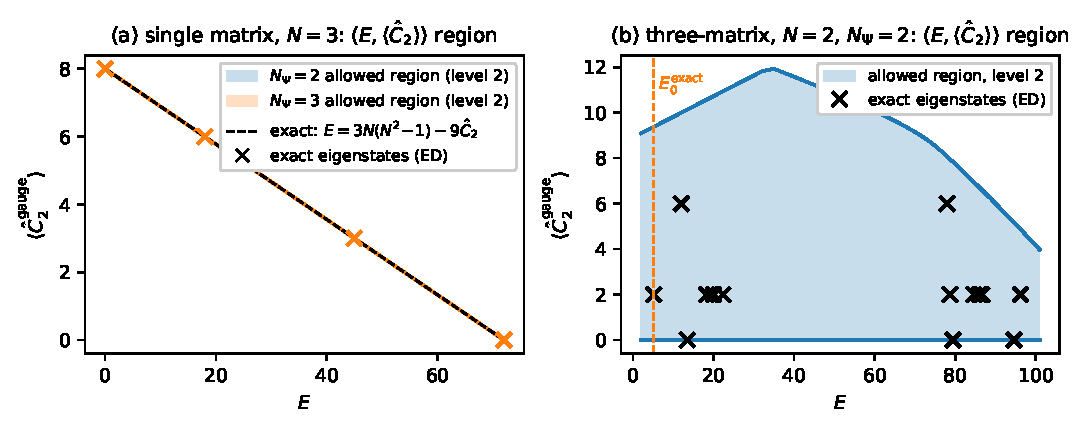
\includegraphics[width=0.78\textwidth]{report_figs/allowed_regions.pdf}
\caption{Allowed regions in the energy and gauge-Casimir plane from the level-2 sector bootstrap, obtained by
fixing $\phi(H)=E$ and extremising $\phi(\hat C_2)$, against the exact eigenstates. (a) Single-matrix model at
$N=3$: the region has zero width and coincides with the exact line $E=3N(N^2-1)-9\hat C_2$, because that
operator identity lies in the span of the constraints. (b) Three-flavour model at $N=2$: a genuine
two-dimensional island, rigorous and already tight at the ground-state edge.}
\label{fig:island}
\end{figure}

Tables \ref{tab:N2} and \ref{tab:largeN} give the sector energies. The bootstrap also produces allowed regions
rather than single numbers. Fixing $\phi(H)=E$ and extremising an observable maps out an island in the
$(E,\langle\hat C_2\rangle)$ plane enclosing the exact spectrum (Fig.~\ref{fig:island}); for the single-matrix
model the island degenerates to the exact Casimir line, which is the cleanest possible illustration of what a
Casimir Hamiltonian does to the constraint span. With eigenstate constraints $\phi(OH)=E\,\phi(O)$ added, the
level-2 problem becomes feasible only at the exact eigenvalues, $5.16536$, $12$ and $13.4907$, each to $10^{-8}$:
an archipelago rather than an island.

\begin{figure}[t]\centering
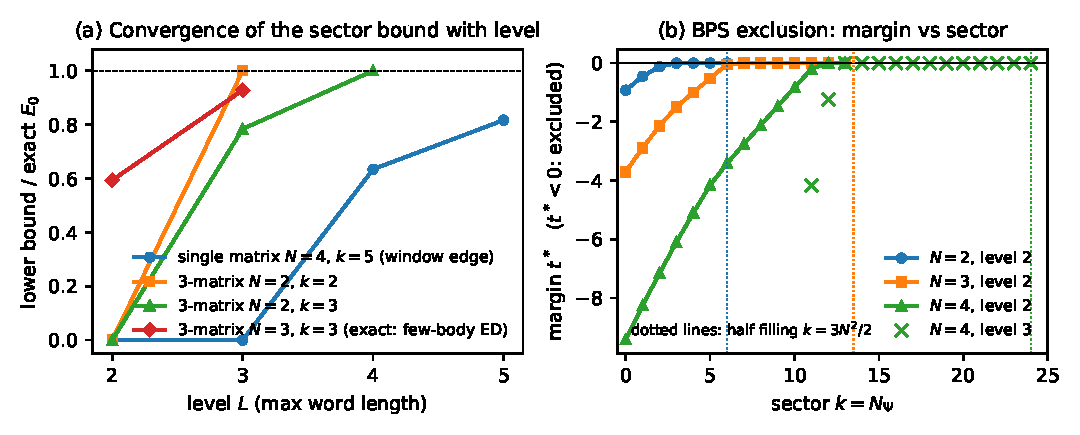
\includegraphics[width=0.78\textwidth]{report_figs/convergence_exclusion.pdf}
\caption{(a) Sector lower bound divided by the exact ground energy as a function of level, for four
representative sectors. (b) BPS-exclusion margin as a function of the sector: a negative margin certifies that
the sector contains no BPS state at that level.}
\label{fig:conv}
\end{figure}

\paragraph{BPS exclusion, and where the two methods meet.}
A BPS state satisfies $Q\psi=\bQ\psi=0$ and therefore $\phi(XQ)=\phi(QX)=\phi(X\bQ)=\phi(\bQ X)=0$ for every
$X$. Adding those rows to \eqref{eq:sdp} and maximising a feasibility margin turns the bootstrap into a
certificate of absence: a negative margin means the sector contains no BPS state. At $N=2$ this excludes
$k\le2$ at level 2 and $k\le3$ at level 3, one level earlier than the energy bound each time; at $N=3$ and $N=4$
level 2 already excludes $k\le6$ and $k\le11$ in seconds (Fig.~\ref{fig:conv}b).

The test sharpens considerably once it is resolved by irrep, which is possible because the gauge Casimir is
itself a trace polynomial (Section \ref{sec:singletrace}), so $\phi((\hat C_2-c_\lambda)X)=0$ is a family of
linear rows of exactly the same type as the sector rows. Table~\ref{tab:exclusion} shows what happens in the
maximal-Casimir irrep, where the largest complexes live.

\begin{table}[t]\centering\small
\begin{tabular}{@{}lcccccc@{}}\toprule
$N=3$, $C_2=48$: \ sector $k$ & 8 & 9 & 10 & 11 & 12 & 13\\
\midrule
exclusion margin & $-0.876$ & $-0.340$ & $-0.050$ & $-0.003$ & $-0.0000$ & $-0.0000$\\
BPS states from exact cohomology & none & none & none & none & $27$ & $81$\\
\bottomrule
\end{tabular}
\caption{The bootstrap meeting the cohomology. In the maximal-Casimir irrep at $N=3$ the BPS-exclusion margin is
clearly negative, hence a certificate of absence, at $k=8,9,10,11$; it then decays to solver tolerance exactly at
$k=12$, which is where the exact computation of Section \ref{sec:numerics} places the lower edge of the window.
The two calculations share no input. At $N=4$ the same test in the $C_2=120$ irrep excludes $k=18,19,20$ and
loses resolution from $k=21$, one sector short of the true edge at $k=22$.}
\label{tab:exclusion}
\end{table}

This is the point of running both methods. The cohomology knows where the window is but says nothing about the
sectors outside it beyond the fact that they are empty; the bootstrap knows nothing about the window but
certifies emptiness sector by sector, and its certificate degrades precisely at the boundary the cohomology
identifies. Neither result depends on the other, and the exclusions never contradict the exact counts, which is
a genuine consistency check on two very different pieces of machinery. It also indicates the limit of the
method as currently implemented: the margins shrink by an order of magnitude per sector as the window is
approached, so reaching the edge from outside requires either higher level or sharper irrep resolution, for
instance through the cubic Casimir, which is also a trace polynomial.

\paragraph{An analytic complement.} Because $Q$ raises $N_\Psi$ by three, the sectors organise into three
strands $\mathcal H_c\to\mathcal H_{c+3}\to\cdots$, each split further by irrep and flavour charge, and the
Euler characteristic of a strand is purely kinematic. Its modulus bounds the number of BPS multiplets below,
with equality exactly when the strand is concentrated. Using $\mathbb Z_3$-Fourier flavour letters the Fock
character $\prod_m\prod_{i,j}(1+tz^mu_i/u_j)$ gives every such index exactly, and the totals per strand have the
closed form
\begin{equation}
I_c(N)=\tfrac23\,3^{3N^2/2}\cos\!\Big(\tfrac{2\pi c}{3}+\tfrac{\pi N^2}{2}\Big),
\end{equation}
which is the Turiaci--Witten profile $\cos(\pi(k-k_*)/3)$ about half filling: $2{:}1{:}1$ for even $N$ and
$0{:}1{:}1$ for odd $N$. The per-irrep multiplicities grow like $e^{0.75N^2}$, being $18$, $891$ and
$3.5\times10^5$ at $N=2,3,4$, and include gauge singlets. The single-matrix model put through the same
computation has a single irrep per strand, multiplicity at most $9$, and no singlets at all.

\subsection{Exact energies up to the window}\label{sec:nearwindow}

The sectors next to the window are the ones the super-Schwarzian question is about, and they are where the
bootstrap is weakest, so we have computed them exactly. The sector $k$ at $N=3$ has dimension $\binom{27}k$, up
to $1.3\times10^7$ at $k=11$, but $H$ commutes with the gauge group and is therefore block diagonal in the weight.
The weight is the vector of Cartan charges $\mu_i$: the number of occupied modes with row index $i$, minus the
number with column index $i$. Every weight in the Fock space is a sum of roots $e_i-e_j$, and an irrep whose
weights lie in the root lattice always contains the zero weight. The lowest eigenvalue of the zero-weight block
is therefore the ground energy of the whole sector. A level of irrep $\lambda$ appears in that block as many
times as $\lambda$ has zero-weight states: once for $\mathbf 1$, $\mathbf{10}$ and $\overline{\mathbf{10}}$,
twice for $\mathbf 8$, three times for $\mathbf{27}$. At $k=11$ the block has $750\,699$ states. We
diagonalised $H$ in these blocks, by Lanczos where they are large and directly where they are small, and named the irrep of each eigenvector from its expectation value
of $\hat C_2$, equation \eqref{eq:casimir}. The implementation and its checks are described in
Appendix~\ref{app:numerics}.

Non-BPS states come in pairs. If $Q\psi\ne0$, then $\psi$ in sector $k$ and $Q\psi$ in sector $k+3$ have the
same energy, since $Q$ commutes with $H$. Following Turiaci and Witten \cite{TW} we label a pair by its
average R-charge, measured from half filling, which is where the particle-hole symmetry $k\to pN^2-k$ puts the
centre:
\begin{equation}
J=k-\frac{pN^2}2,\qquad q=\tfrac12\big(J_k+J_{k+3}\big)=k+\frac32-\frac{pN^2}2 .
\label{eq:multipletq}
\end{equation}
The ground state $\psi$ of a sector below the window is always the lower member of its pair. If $\bQ\psi$ were
non-zero it would be an eigenstate of energy $E_0(k)$ in sector $k-3$, whereas every computed ground energy
satisfies $E_0(k-3)>E_0(k)$. Hence $\bQ\psi=0$, so $\psi=\bQ Q\psi/E_0(k)$ and $Q\psi\ne0$. The partner sits in
sector $k+3$, and $|q|=pN^2/2-k-3/2$ measures how far the pair lies from half filling: an integer at $N=3$, a
half-integer at $N=2$. At $N=3$, for example, the ground state of $k=11$ pairs with a state of $k=14$, so
$J=-\tfrac52,\tfrac12$ and $q=-1$.

\begin{table}[t]\centering\small
\begin{tabular}{@{}cccrll@{}}\toprule
$N$ & $k$ & $|q|$ & block & $E_0(k;N)$, irrep & next levels (irrep)\\\midrule
2 & 2 & 2.5 & 24 & 5.16536, $\mathbf 3$ & 12.00 ($\mathbf 5$), 13.49 ($\mathbf 1$)\\
2 & 3 & 1.5 & 74 & 1.22706, $\mathbf 1$ & 1.552 ($\mathbf 5$), 1.965 ($\mathbf 3$)\\
2 & 4 & 0.5 & 159 & 0.087961, $\mathbf 1$ & 0.226 ($\mathbf 5$), 0.357 ($\mathbf 3$)\\\midrule
3 & 6 & 6 & 23\,388 & 12.5602, $\mathbf{10}\oplus\overline{\mathbf{10}}$ & 16.14 ($\mathbf{64}$), 16.16 ($\mathbf{27}$)\\
3 & 7 & 5 & 63\,486 & 6.63510, $\mathbf 8$ & 8.19 ($\mathbf{35}\oplus\overline{\mathbf{35}}$), 8.32 ($\mathbf{10}\oplus\overline{\mathbf{10}}$)\\
3 & 8 & 4 & 146\,943 & 2.73751, $\mathbf 1$ & 3.634 ($\mathbf 8$), 3.739 ($\mathbf{27}$)\\
3 & 9 & 3 & 292\,179 & 1.14573, $\mathbf 1$ & 1.497 ($\mathbf 8$), 1.713 ($\mathbf{27}$)\\
3 & 10 & 2 & 502\,245 & 0.345019, $\mathbf 8$ & 0.464 ($\mathbf{10}\oplus\overline{\mathbf{10}}$), 0.471 ($\mathbf{64}$)\\
3 & 11 & 1 & 750\,699 & 0.061408, $\mathbf{10}\oplus\overline{\mathbf{10}}$ & 0.0651 ($\mathbf 8$), 0.0696 ($\mathbf{10}\oplus\overline{\mathbf{10}}$), 0.0710 ($\mathbf{27}$)\\
\bottomrule
\end{tabular}
\caption{Exact ground energies of the sectors below the window, from diagonalisation of the zero-weight block,
whose dimension is given (Lanczos for the blocks above $3000$), with $|q|$ from \eqref{eq:multipletq}. Irreps are named by dimension and
identified from $\langle\hat C_2\rangle$. The $\mathbf{10}$ and $\overline{\mathbf{10}}$ share a Casimir and are
exactly degenerate, as are $\mathbf{35}$ and $\overline{\mathbf{35}}$. The sectors $k\le1$ at $N=2$ and $k\le2$
at $N=3$ are free, \eqref{eq:free}, and the windows are $k=5\ldots7$ and $k=12\ldots15$.}
\label{tab:nearwindow}
\end{table}

\begin{figure}[t]\centering
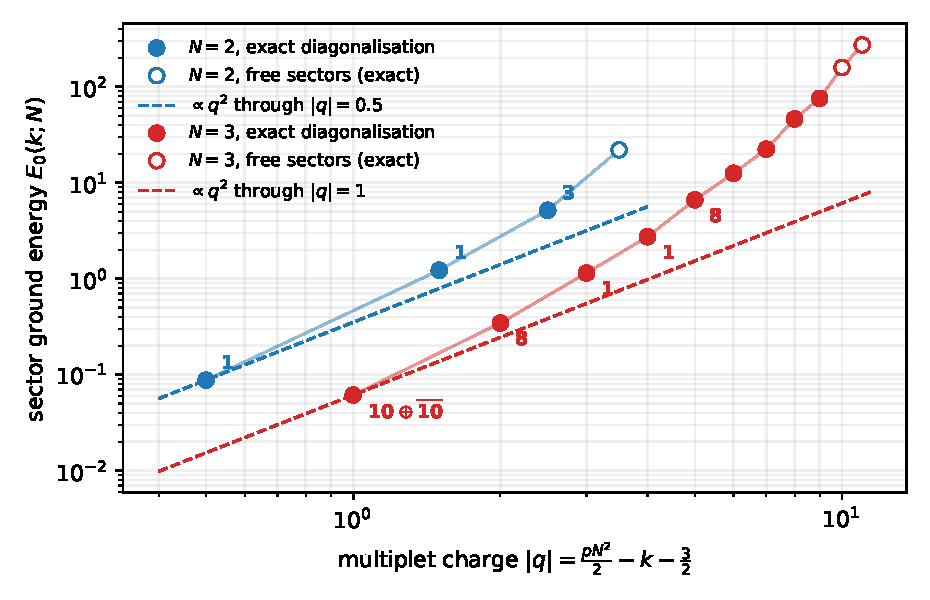
\includegraphics[width=0.74\textwidth]{report_figs/near_window_gaps.pdf}
\caption{Sector ground energies below the window against the multiplet charge $|q|$ of \eqref{eq:multipletq}, at
$N=2$ and $3$, from exact diagonalisation of the zero-weight block of each sector. Open circles are free sectors,
given exactly by \eqref{eq:free}. The dashed lines are the super-Schwarzian law $E_0\propto q^2$, drawn through
the point nearest the window. The labels give the irrep of each ground state near the window.}
\label{fig:nearwindow}
\end{figure}

Table~\ref{tab:nearwindow} and Fig.~\ref{fig:nearwindow} show the result. At $N=3$ the ground energy falls by a
factor of more than $4000$ between $k=1$ and $k=11$, to $E_0(11;3)=0.0614$. The ground states near the window
lie in irreps of small Casimir, and which one wins changes from sector to sector: a singlet at $k=8$ and $9$, the
adjoint at $k=10$, and $\mathbf{10}\oplus\overline{\mathbf{10}}$ at $k=11$, where the four lowest levels lie
within $16\%$ of one another. The pairing of each irrep with its conjugate is exact. Transposing every matrix
while exchanging flavours $1$ and $3$ sends $Q$ to $-Q$: reversing three fermions inside a trace costs a sign,
and the exchange maps the reversed couplings back to themselves. This operation therefore commutes with $H$,
and since transposition negates every weight, it maps each irrep to its conjugate.

The maximal irrep plays no part in this. On its weight space every mode $\Psi^a_{ij}$ with $i<j$ is filled and
every mode with $i>j$ is empty. A term of $Q$ or $\bQ$ moves three modes of total weight zero, so if it touches
an off-diagonal mode it touches one of each kind, and it vanishes on this space: creating a filled mode or
annihilating an empty one gives zero. Only the diagonal modes $\psi^a_i=\Psi^a_{ii}$ act, through
$Q=\sum_iq_i$ with $q_i=\psi^1_i\psi^2_i\psi^3_i$ for the three-flavour couplings. Odd operators on different
sites anticommute, so on this space $H=\sum_i\{q_i,\bar q_i\}$. These are $N$ independent sites, each costing
one unit of energy when it is empty or full. The spectrum of $H$ in the maximal irrep is exactly
$\{0,1,\dots,N\}$, with a gap of one next to the window at every $N$; diagonalising every sector at $N=2,3$
confirms this level by level. The energies of Fig.~\ref{fig:nearwindow}, which fall far below one, all come
from irreps of small Casimir.

The super-Schwarzian predicts $E_0(q)=q^2/(4\hat q^2)$ in its own units \cite{TW}, so $E_0/q^2$ should be
constant. The data rise faster. Between neighbouring points the slope $d\ln E_0/d\ln|q|$ is $2.4$ at $N=2$ and
$2.5$ at $N=3$ next to the window, and it grows outward. At comparable $|q|$ the energies at $N=3$ are an order
of magnitude below those at $N=2$, while the vacuum energy grows fourfold. This is not yet a test of the law,
which is a large-$N$ statement about a model whose BPS states occupy $\hat q=3$ charges, whereas at $N=3$ they
occupy four, and two values of $N$ do not determine a scaling. What the computation supplies is exact targets
for the bootstrap in the sectors where it is weakest.

\section{Single-trace formulas for $H$, $Q$ and $\hat C_2$}\label{sec:singletrace}

\subsection{The Hamiltonian}

Both the trace bootstrap and the Casimir-resolved exclusion need $H$ and $\hat C_2$ as explicit trace
polynomials. Writing $Q=C_{abc}\Tr[\Psi^a\Psi^b\Psi^c]$ with $C$ cyclic, defining the flavour tensors
\begin{equation}
K_{bc;ed}=\sum_aC_{abc}\bar C_{dea},\quad M_{cd}=\sum_{ab}C_{abc}\bar C_{abd},\quad
L_{cd}=\sum_{ab}C_{abc}\bar C_{bad},\quad \|C\|^2=\sum|C_{abc}|^2,
\end{equation}
and the matrix-valued composites $X_a=C_{abc}\Psi^b\Psi^c$, a Wick expansion of the anticommutator gives the
normal-ordered canonical form
\begin{equation}
H=\{Q,\bQ\}=9\sum_a\Tr[X_a\bar X_a]\;-\;9N\,M_{cd}\,\Tr[\Psi^c\bPsi^d]\;+\;9\,L_{cd}\,\Tr\Psi^c\,\Tr\bPsi^d
\;+\;3N^3\|C\|^2-3N\langle C,C^{\rm rev}\rangle .
\label{eq:Hgeneral}
\end{equation}
The structure is a single-trace quartic, a single-trace quadratic, a product of two length-one traces, and a
constant. The quartic is the normal-ordered $|\partial Q|^2$, as it must be for $\{Q,\bQ\}$ with $Q$ built from
creation operators only. The only genuine double trace is $\Tr\Psi^c\Tr\bPsi^d$, a bilinear in the $p$
trace-mode fermions, of size $O(N)$ against the $O(N^3)$ of the other terms and therefore suppressed by
$1/N^2$, though we keep it exactly at finite $N$. This was verified as an operator identity on random vectors to
relative residual $8\times10^{-16}$ at $(N,p)=(2,1),(3,1),(2,2),(3,2),(2,3)$.

Specialising to the three-flavour model, $\|C\|^2=16/3$, $\langle C,C^{\rm rev}\rangle=5$,
$M=\frac59\mathbb 1+\frac{11}9\mathbb J$ and $L=\frac49\mathbb 1+\frac{11}9\mathbb J$, so
\begin{equation}
H=9\sum_{a=1}^3\Tr[X_a\bar X_a]-5N\,N_\Psi-11N\sum_{c,d}\Tr[\Psi^c\bPsi^d]
+4\sum_c\Tr\Psi^c\Tr\bPsi^c+11\sum_{c,d}\Tr\Psi^c\Tr\bPsi^d+16N^3-15N .
\label{eq:H3}
\end{equation}
Reading off the vacuum energy gives $E_0(0)=E_0(3N^2)=16N^3-15N$, which is $98$ at $N=2$ and $387$ at $N=3$, and
the one-particle sector gives gauge-traceless states at $16N^3-53N$ and $16N^3-20N$ and trace-mode states at
$16N^3-16N$. These are the analytic anchors used to validate the bootstrap in Section \ref{sec:bootstrap}. Note
also that the trace modes do not decouple at $p=3$ as they do at $p=1$: expanding $\Psi^a$ into trace and
traceless parts, $Q$ retains a term proportional to $C_{a[bc]}$, which is non-zero for the three-flavour
couplings, so the $\su(N)$ version of the model is a genuinely different theory.

\subsection{The gauge Casimir}

Under $\Psi^a\to U\Psi^aU^\dagger$ the one-body generator for traceless $T$ is $E(T)=\sum_{ii'}T_{ii'}M_{ii'}$
with the matrix word $M=\sum_a(\Psi^a\bPsi^a+\bPsi^a\Psi^a)$, and the completeness relation for $su(N)$ gives
\begin{equation}
\hat C_2=\sum_xJ^xJ^x=\tfrac12\Tr[M^2]-\frac{(\Tr M)^2}{2N}
=\tfrac12\sum_{a,b}\Tr\big[(\Psi^a\bPsi^a+\bPsi^a\Psi^a)(\Psi^b\bPsi^b+\bPsi^b\Psi^b)\big]-\tfrac12p^2N^3 ,
\label{eq:casimir}
\end{equation}
a trace polynomial of degree four, flavour invariant, with eigenvalue
$c_\lambda=\frac12\sum_i\lambda_i(\lambda_i+N+1-2i)$ on the irrep $\lambda$. This was verified against the
explicit $\sum_xJ^xJ^x$ to $10^{-16}$ at $(N,p)=(2,3),(2,1),(3,1)$. Equation \eqref{eq:casimir} is what makes the
irrep-resolved exclusion of Table~\ref{tab:exclusion} possible: a functional supported on the $\hat C_2=c_\lambda$
eigenspace obeys $\phi((\hat C_2-c_\lambda)X)=0$, linear rows of the same form as the sector rows.

\subsection{Why the model is not Casimir-solvable}

For a single flavour, $H=3N(N^2-1)-9\hat C_2$ and everything is determined by representation theory. That
mechanism is gone at $p=3$, and in two independent ways. Structurally, the quartic part $9K_{bc;ed}V^{bced}$
contains no alternating words $\Tr[\Psi\bPsi\Psi\bPsi]$, while \eqref{eq:casimir} does, and $K$ is not
proportional to the Casimir flavour structure: projecting it gives the component $-\frac{16}{3}\hat C_2$ against
$-9\hat C_2$ at $p=1$, but the remainder is non-zero. Numerically at $N=2$, resolving $N_\Psi$, $\hat C_2$, $J_z$
and the $\mathbb Z_3$ charge simultaneously splits the $4096$-dimensional space into $353$ joint sectors, and in
$245$ of them the restriction of $H$ has more than one distinct eigenvalue, which a function of Casimirs cannot.
The same computation shows the commutant of $H$ among one-body operators is exactly four-dimensional,
$\mathrm{span}(J^1,J^2,J^3,N_\Psi)$, so there is no hidden continuous symmetry and in particular no conserved
flavour charge.

This is the reason the bootstrap of Section \ref{sec:bootstrap} has to be sector-resolved. When $H$ is a Casimir
function the operator identity lies in the span of the constraints, the allowed region collapses to a line
(Fig.~\ref{fig:island}a), and nothing has to be solved. When it is not, $E_0(N_\Psi,\lambda)$ is a genuine
dynamical quantity, the supersymmetric floor $\phi(H)\ge0$ has to be lifted by constraints that actually see the
sector, and the island acquires two dimensions (Fig.~\ref{fig:island}b). It is also the reason $p=3$ was singled
out in the first place: it is the smallest flavour number for which the Casimir shortcut fails, and our own
cohomology confirms the same transition from a different direction, since at $p=1$ the BPS states occupy a single
irrep while at $p\ge2$ they are spread over every irrep the Fock space contains.

\section{Status}

The exact side is in good shape at the top of the spectrum and thins out below it. The rank law
\eqref{eq:ranklaw} and the trichotomy \eqref{eq:trichotomy} are derived; the lower bound \eqref{eq:main} is
derived and tight for $p\le3$; the irrep-resolved spectra of Table~\ref{tab:cohom} are exact but reach only
thirteen irreps at $N=3$ and $N=4$, and the complexes with genuinely macroscopic index, which is what the
concentration conjecture is about, remain out of reach without a sparse exact rank routine. Two statements are
verified rather than proved: that the window is the same in every irrep, and that a generic $q$-form saturates
its index class by class.

The bootstrap side is rigorous wherever it returns a number, but its reach is set by the level. At $N=2$ it is
exact in every gapped sector except the almost-BPS sector $k=4$, where $E_0=0.08796$ and the bound has not left
zero by level 4; it gives \eqref{eq:free} for the free sectors at any $N$, and one rigorous bound in an
interacting sector beyond $N=2$. The immediate next step is the level-4 problem, which is assembled but not yet
solved to tolerance. The question the project is ultimately after lies elsewhere. A super-Schwarzian tail is a
statement about the lightest non-BPS states in and next to the BPS window, which sits near half filling,
$k\approx pN^2/2$, not in the low sectors the bootstrap now controls. Exact diagonalisation now gives every
sector energy up to the window at $N=3$ (Section \ref{sec:nearwindow}). There the energy next to the window
drops by an order of magnitude from $N=2$, the near-window states lie in irreps of small Casimir, and the energies
rise faster than the $q^2$ law away from the window, though two values of $N$ do not determine a scaling. In
these sectors the bootstrap has so far produced no energy bound above zero, only the certificates of absence of
Table~\ref{tab:exclusion}, so matching them is the next test of the method.

\appendix
\section{Numerical implementation}\label{app:numerics}

\paragraph{Finite-$N$ engine.} Open words are built as blocks between sectors, so the $2^{pN^2}$-dimensional
space is never formed. An isotypic reducer maps every operator to its $D=\sum_Rm_R^2$ invariant components as
soon as it is built, and the spans of the touched operators and of the equations of motion are accumulated as
streaming $2D\times2D$ Gram matrices. A diagnostic that evaluates every constraint on the exact,
multiplet-averaged ground state caught a round-off Hermitian part being normalised into a spurious constraint;
all such cutoffs are now relative to $\|X\|$.

\paragraph{Trace algebra.} One primitive generates everything: swapping two adjacent letters in a routed term,
meaning letters in operator order together with a routing permutation, where the anticommutator branch rewires
the routing and closed index loops give factors of $N$. From it follow canonical cyclic forms, products,
daggers, commutators with $H$, self-symmetry reductions such as $\Tr[\ell\ell]=0$, and the finite-$N$ relations
from the vanishing antisymmetriser over $N+1$ indices. Coefficients are polynomials in $N$. Every identity is
checked against explicit operators at $N=2,3$, a thousand random terms to $10^{-15}$, and the algebra recovers
$\{Q,\bQ\}=H$ on its own.

\paragraph{Assembly and conditioning.} Variables are generated by closure; reality is imposed at the variable
level, halving the unknowns; rows are unit-normalised; the unknowns carry a 't~Hooft scaling
$N^{\sum(1+L_i/2)}$ and the objective is divided by $N^3$, without which nothing works beyond $N\approx30$.
Solvers are called directly. The settings that matter are Clarabel with chordal decomposition off and
equilibration on, and SCS with $\rho_x=10^{-3}$, the Apple-Accelerate LDL backend and fixed scaling. A parallel
fixed-$N$ build produces the level-4 problem, $51$k monomials with cones up to dimension $168$, in $25$ seconds.

\paragraph{Exact cohomology.} For Section \ref{sec:numerics}, ranks are computed over $\mathbb F_P$ with
$P=2^{31}-1$ and cross-checked against $P'=2147483629$. The blocked routine uses a prime small enough that
$b(P-1)^2<2^{53}$, so that a float64 matrix multiply of inner dimension $b$ is exact integer arithmetic and can
be reduced afterwards; this makes the trailing update of the elimination a single BLAS call. Flavour blocking
over a field containing a $p$-th root of unity splits each weight space into $p$ blocks. The largest weight
space handled is $30\,294$ after blocking, in about thirty minutes at $6.1$ GB.

\paragraph{Exact diagonalisation.} For Section \ref{sec:nearwindow} the zero-weight basis of each sector is
enumerated by the same pruned search over occupation matrices used for the cohomology, and stored as 64-bit
occupation masks. The Hamiltonian is assembled as $H=16N^3-15N+H_1+9\,Y^\dagger Y$. Here $H_1$ is the quadratic
part of \eqref{eq:Hgeneral}, and $Y$ stacks the pair-annihilation operators $\big((X_a)_{ik}\big)^\dagger$, with
one row for each $(a,i,k)$ and each $(k-2)$-particle state reached, so that $9\,Y^\dagger Y$ is the quartic term.
Every operator is built by vectorised bit operations, with the Jordan--Wigner signs from population counts.
Storing $Y$ rather than its square keeps the cost at about $k(k-1)$ entries per state. At $N=3$, $k=11$ this is
$7.5\times10^7$ entries; the build takes ten seconds, the Lanczos run (ARPACK, twelve eigenvalues, residuals below
$10^{-11}$) forty minutes, and the peak memory is $3$ GB. Three checks guard the result. Each run compares
$\langle v|H|v\rangle$ with $\|Qv\|^2+\|\bQ v\|^2$, computed from the supercharge directly, on a random vector, and
the two agree to $10^{-12}$. An independent pure-Python construction gives identical spectra at $k=8,9$. The
method reproduces the full diagonalisation at $N=2$ and the free values \eqref{eq:free}. The Casimir labels use the
one-body gauge generators on the computed eigenvectors. Lanczos can miss copies of an exactly degenerate level,
so degeneracies are read from the irrep labels rather than counted.

\section{Irreps and cohomology, irrep by irrep}\label{app:irreps}

The tables below list the $U(N)$ content of the $p=3$ Fock space: every occurring highest weight $\lambda$, its
quadratic Casimir, the dimension $\dim V_\lambda$ of the irrep, its multiplicity in the full Fock space, and,
where we have computed it, the exact BPS cohomology. Occurrence is governed by dominance, $\lambda\le\lambda^*$,
which is stricter than the box bound $|\lambda_i|\le p(N-1)$ and was checked against the Weyl alternating sum.
Multiplicities are cross-checked the same way. The number of BPS \emph{states} carried by an irrep is
$\dim V_\lambda$ times the multiplicity $h^k$ summed over $k$, so the small irreps at low Casimir dominate the
totals quoted in Table~\ref{tab:cohom} even though their multiplicities per degree are modest.

Two points are visible in the tables and not in the summary. The window is literally the same set of degrees in
every irrep reached, not merely the same width, and this persists a long way down the Casimir ladder. And the
profile is not universal: at $N=4$ it is $81\binom4j$ in eleven of the thirteen computed irreps and differs in
the twelfth and thirteenth, so the width is the robust statement and the shape is not.

\begin{table}[p]\centering\small
\begin{tabular}{rlrrrll}
\toprule
\# & $\lambda$ & $C_2$ & $\dim V_\lambda$ & Fock mult. & window & BPS multiplets $h^k$\\
\midrule
1 & $(3,-3)$ & 12 & 7 & 64 & $5\ldots7$ & 9, 18, 9\\
2 & $(2,-2)$ & 6 & 5 & 320 & $5\ldots7$ & 18, 36, 18\\
3 & $(1,-1)$ & 2 & 3 & 576 & $5\ldots7$ & 27, 54, 27\\
4 & $(0,0)$ & 0 & 1 & 320 & $5\ldots7$ & 9, 18, 9\\
\bottomrule\end{tabular}
\caption{$N=2$, $p=q=3$: all four irreps of the Fock space, each with exact BPS cohomology. The window is $5\ldots7$ throughout, and $\sum_\lambda(\dim V_\lambda)(\sum_kh^k)=972$ reproduces the full exact diagonalisation.}\label{tab:app2}
\end{table}

\begin{table}[p]\centering\small
\begin{tabular}{rlrrrll}
\toprule
\# & $\lambda$ & $C_2$ & $\dim V_\lambda$ & Fock mult. & window & BPS multiplets $h^k$\\
\midrule
1 & $(6,0,-6)$ & 48 & 343 & 512 & $12\ldots15$ & 27, 81, 81, 27\\
2 & $(5,1,-6)$ & 42 & 260 & 2\,560 & $12\ldots15$ & 54, 162, 162, 54\\
3 & $(6,-1,-5)$ & 42 & 260 & 2\,560 & $12\ldots15$ & 54, 162, 162, 54\\
4 & $(4,2,-6)$ & 38 & 162 & 4\,608 & $12\ldots15$ & 81, 243, 243, 81\\
5 & $(6,-2,-4)$ & 38 & 162 & 4\,608 & $12\ldots15$ & 81, 243, 243, 81\\
6 & $(3,3,-6)$ & 36 & 55 & 2\,560 & $12\ldots15$ & 27, 81, 81, 27\\
7 & $(6,-3,-3)$ & 36 & 55 & 2\,560 & $12\ldots15$ & 27, 81, 81, 27\\
8 & $(5,0,-5)$ & 35 & 216 & 15\,360 & $12\ldots15$ & 38, 486, 486, 38\\
9 & $(4,1,-5)$ & 30 & 154 & 35\,840 & $12\ldots15$ & 36, 810, 810, 36\\
10 & $(5,-1,-4)$ & 30 & 154 & 35\,840 & $12\ldots15$ & 36, 810, 810, 36\\
11 & $(3,2,-5)$ & 27 & 80 & 35\,840 & $12\ldots15$ & 18, 648, 648, 18\\
12 & $(5,-2,-3)$ & 27 & 80 & 35\,840 & $12\ldots15$ & 18, 648, 648, 18\\
13 & $(4,0,-4)$ & 24 & 125 & 110\,080 & $12\ldots15$ & 64, 1\,620, 1\,620, 64\\
14 & $(3,1,-4)$ & 20 & 81 & 161\,280 & -- & \emph{not computed}\\
15 & $(4,-1,-3)$ & 20 & 81 & 161\,280 & -- & \emph{not computed}\\
16 & $(2,2,-4)$ & 18 & 28 & 82\,432 & -- & \emph{not computed}\\
17 & $(4,-2,-2)$ & 18 & 28 & 82\,432 & -- & \emph{not computed}\\
18 & $(3,0,-3)$ & 15 & 64 & 337\,920 & -- & \emph{not computed}\\
19 & $(2,1,-3)$ & 12 & 35 & 322\,560 & -- & \emph{not computed}\\
20 & $(3,-1,-2)$ & 12 & 35 & 322\,560 & -- & \emph{not computed}\\
21 & $(2,0,-2)$ & 8 & 27 & 511\,488 & -- & \emph{not computed}\\
22 & $(1,1,-2)$ & 6 & 10 & 268\,800 & -- & \emph{not computed}\\
23 & $(2,-1,-1)$ & 6 & 10 & 268\,800 & -- & \emph{not computed}\\
24 & $(1,0,-1)$ & 3 & 8 & 359\,424 & -- & \emph{not computed}\\
25 & $(0,0,0)$ & 0 & 1 & 74\,240 & -- & \emph{not computed}\\
\bottomrule\end{tabular}
\caption{$N=3$, $p=q=3$: all 25 occurring irreps. Cohomology is exact in the thirteen with $C_2\ge24$, and the window is $12\ldots15$ in every one of them, including $(4,0,-4)$ whose Fock multiplicity is some $215$ times that of the maximal irrep. The twelve below $C_2=24$ have weight spaces up to $1.1\times10^6$ and need a sparse rank routine.}\label{tab:app3}
\end{table}

\begin{table}[p]\centering\small
\begin{tabular}{rlrrrll}
\toprule
\# & $\lambda$ & $C_2$ & $\dim V_\lambda$ & Fock mult. & window & BPS multiplets $h^k$\\
\midrule
1 & $(9,3,-3,-9)$ & 120 & 117\,649 & 4\,096 & $22\ldots26$ & 81, 324, 486, 324, 81\\
2 & $(8,4,-3,-9)$ & 114 & 91\,000 & 20\,480 & $22\ldots26$ & 162, 648, 972, 648, 162\\
3 & $(9,2,-2,-9)$ & 114 & 94\,640 & 20\,480 & $22\ldots26$ & 162, 648, 972, 648, 162\\
4 & $(9,3,-4,-8)$ & 114 & 91\,000 & 20\,480 & $22\ldots26$ & 162, 648, 972, 648, 162\\
5 & $(7,5,-3,-9)$ & 110 & 57\,456 & 36\,864 & $22\ldots26$ & 243, 972, 1\,458, 972, 243\\
6 & $(9,1,-1,-9)$ & 110 & 61\,236 & 36\,864 & $22\ldots26$ & 243, 972, 1\,458, 972, 243\\
7 & $(9,3,-5,-7)$ & 110 & 57\,456 & 36\,864 & $22\ldots26$ & 243, 972, 1\,458, 972, 243\\
8 & $(6,6,-3,-9)$ & 108 & 19\,635 & 20\,480 & $22\ldots26$ & 81, 324, 486, 324, 81\\
9 & $(8,4,-4,-8)$ & 108 & 69\,825 & 102\,400 & $22\ldots26$ & 324, 1\,296, 1\,944, 1\,296, 324\\
10 & $(9,0,0,-9)$ & 108 & 21\,175 & 20\,480 & $22\ldots26$ & 81, 324, 486, 324, 81\\
11 & $(9,3,-6,-6)$ & 108 & 19\,635 & 20\,480 & $22\ldots26$ & 81, 324, 486, 324, 81\\
12 & $(8,3,-2,-9)$ & 107 & 80\,640 & 122\,880 & $22\ldots26$ & 114, 1\,572, 2\,916, 1\,572, 114\\
13 & $(9,2,-3,-8)$ & 107 & 80\,640 & 122\,880 & $22\ldots26$ & 114, 1\,572, 2\,916, 1\,572, 114\\
\midrule
\multicolumn{7}{l}{\emph{remaining 200 irreps, $C_2$ from 104 down to 0, total Fock multiplicity 141\,637\,816\,320: not computed}}\\
\bottomrule\end{tabular}
\caption{$N=4$, $p=q=3$: the thirteen irreps with $C_2\ge107$ for which cohomology is exact, out of 213 occurring. The window is $22\ldots26$ in all of them. The profile $81\binom4j$ holds in eleven and breaks at $C_2=107$, where the edges are suppressed and the centre is unchanged.}\label{tab:app4}
\end{table}

\begin{table}[p]\centering\small
\begin{tabular}{rlrrrll}
\toprule
\# & $\lambda$ & $C_2$ & $\dim V_\lambda$ & Fock mult. & window & BPS multiplets $h^k$\\
\midrule
1 & $(12,6,0,-6,-12)$ & 240 & 282\,475\,249 & n/a & $35\ldots40$ & 243, 1\,215, 2\,430, 2\,430, 1\,215, 243\\
\midrule
\multicolumn{7}{l}{\emph{remaining 2130 irreps, $C_2$ from 234 down to 0: not computed}}\\
\bottomrule\end{tabular}
\caption{$N=5$, $p=q=3$: the maximal irrep, the only one reached, out of 2131 occurring. Fock multiplicities are not tabulated at this size, the Fock space having $2^{75}$ states.}\label{tab:app5}
\end{table}

\begin{thebibliography}{9}\small
\bibitem{Chen} Y.~Chen, \emph{Revisiting fortuity in matrix models}, 2025.
\bibitem{CCSY} C.~Chang, Y.~Chen, W.~Sia, S.~Yang, \emph{Fortuity in SYK models}, 2024.
\bibitem{ChangLin} C.~Chang, Y.~Lin, \emph{Words to describe fortuitous states}, 2024.
\bibitem{FGMS} W.~Fu, D.~Gaiotto, J.~Maldacena, S.~Sachdev, \emph{Supersymmetric SYK models},
Phys.\ Rev.\ D \textbf{95} (2017) 026009.
\bibitem{Cho} M.~Cho, B.~Gabai, J.~Sandor, X.~Yin, \emph{Thermal bootstrap of matrix quantum mechanics}, 2024.
\bibitem{Tierz} M.~Tierz, \emph{BPS spectra of $\mathrm{Tr}[\Psi^p]$ matrix models for odd $p$},
arXiv:2604.27164, 2026.
\bibitem{TW} G.~Turiaci, E.~Witten, \emph{$\mathcal N=2$ JT supergravity and matrix models}, 2023.
\bibitem{Kostant} B.~Kostant, \emph{Eigenvalues of a Laplacian and commutative Lie subalgebras}, Topology
\textbf{3}, suppl.~2 (1965) 147--159.
\bibitem{Schur} I.~Schur, \emph{Zur Theorie der vertauschbaren Matrizen}, J.\ reine angew.\ Math.\ \textbf{130}
(1905) 66--76; N.~Jacobson, \emph{Schur's theorems on commutative matrices}, Bull.\ AMS \textbf{50} (1944)
431--436.
\end{thebibliography}

\end{document}
